\documentclass{article}
\usepackage[utf8]{inputenc}
\usepackage{amssymb, amsmath, amsthm, amsfonts}
\usepackage{thmtools, mathtools, mathrsfs}
\usepackage{forloop}
\usepackage[sort&compress,numbers]{natbib}
\usepackage{subcaption}
\usepackage{graphicx}
\usepackage{caption}
\usepackage{float}
\usepackage{bm}
\pdfminorversion=6

\newcommand{\mb}[1]{\mathbb{#1}}
\newcommand{\mc}[1]{\mathcal{#1}}
\DeclareMathOperator{\Inv}{Inv}
\DeclareMathOperator{\innt}{int}
\DeclareMathOperator{\relu}{ReLU}
\newcommand{\dm}[1]{\ensuremath{\mathrm{d}{#1}}} % dx dy dz dmu
\newcommand{\RN}[2]{\frac{\dm{#1}}{\dm{#2}}} % (Radon-Nikodym) derivative
\newcommand{\PD}[2]{\frac{\partial #1}{\partial #2}} % partial derivative
\newcommand{\overbar}[1]{\mkern 1.5mu\overline{\mkern-1.5mu#1\mkern-1.5mu}\mkern 1.5mu}
\newcommand{\win}{\vW_{\text{in}}}
\newcommand{\wout}{\vW_{\text{out}}}
\newcommand{\bout}{\vb_{\text{out}}}
\newcommand{\reals}{\mathbb{R}}
\newcommand{\defvec}[1]{\expandafter\newcommand\csname v#1\endcsname{{\mathbf{#1}}}}
\newcounter{ct}
\forLoop{1}{26}{ct}{
    \edef\letter{\alph{ct}}
    \expandafter\defvec\letter
}

% captial \vA
\forLoop{1}{26}{ct}{
    \edef\letter{\Alph{ct}}
    \expandafter\defvec\letter
}

\usepackage{tikz}
\usetikzlibrary{positioning,matrix,arrows,decorations.pathmorphing}
\usepackage{tikz-cd} 
% \usetikzlibrary{graphs,graphdrawing,arrows.meta}
% \usegdlibrary{circular}
\definecolor {processblue}{cmyk}{0.8,0,0,0}
\DeclareGraphicsExtensions{.pdf,.png,.jpg,.mps,.eps,.ps}
\graphicspath{{figures/}}
\graphicspath{{../Stability/figures/}}

\newtheorem{theorem}{Theorem}
\newtheorem{prop}{Proposition}
\theoremstyle{definition}
\newtheorem{definition}{Definition}
\theoremstyle{remark}
\newtheorem{remark}{Remark}

\title{Additional Figures}
\author{\'Abel S\'agodi}
\date{15 April 2024}

\begin{document}

\maketitle

\section{Two kinds of continuous attractors}
We found that in the space of RNNs, some have neighbourhoods with highly undesirable exploding gradients. We will describe some continuous attractors which have such neighbourhoods.
Consider an RNN (without input or output for now) expressed in continuous time as an ordinary differential equation:
\begin{align}\label{eq:TLN}
    \dot{\vx} = -\vx + \left[ \vW \vx + \vb \right]_{+}
\end{align}
where $\vx \in \reals^d$ is the hidden state of the network, $\vb > 0$ is the bias, and $[\cdot]_{+} = \max(0,\cdot)$ is the threshold nonlinearity per unit.
In discrete time, this corresponds to a ReLU RNN.
The non-trivial activity of this network is limited to the (non-negative) first quadrant.
\begin{figure}[tbhp]
  \centering
  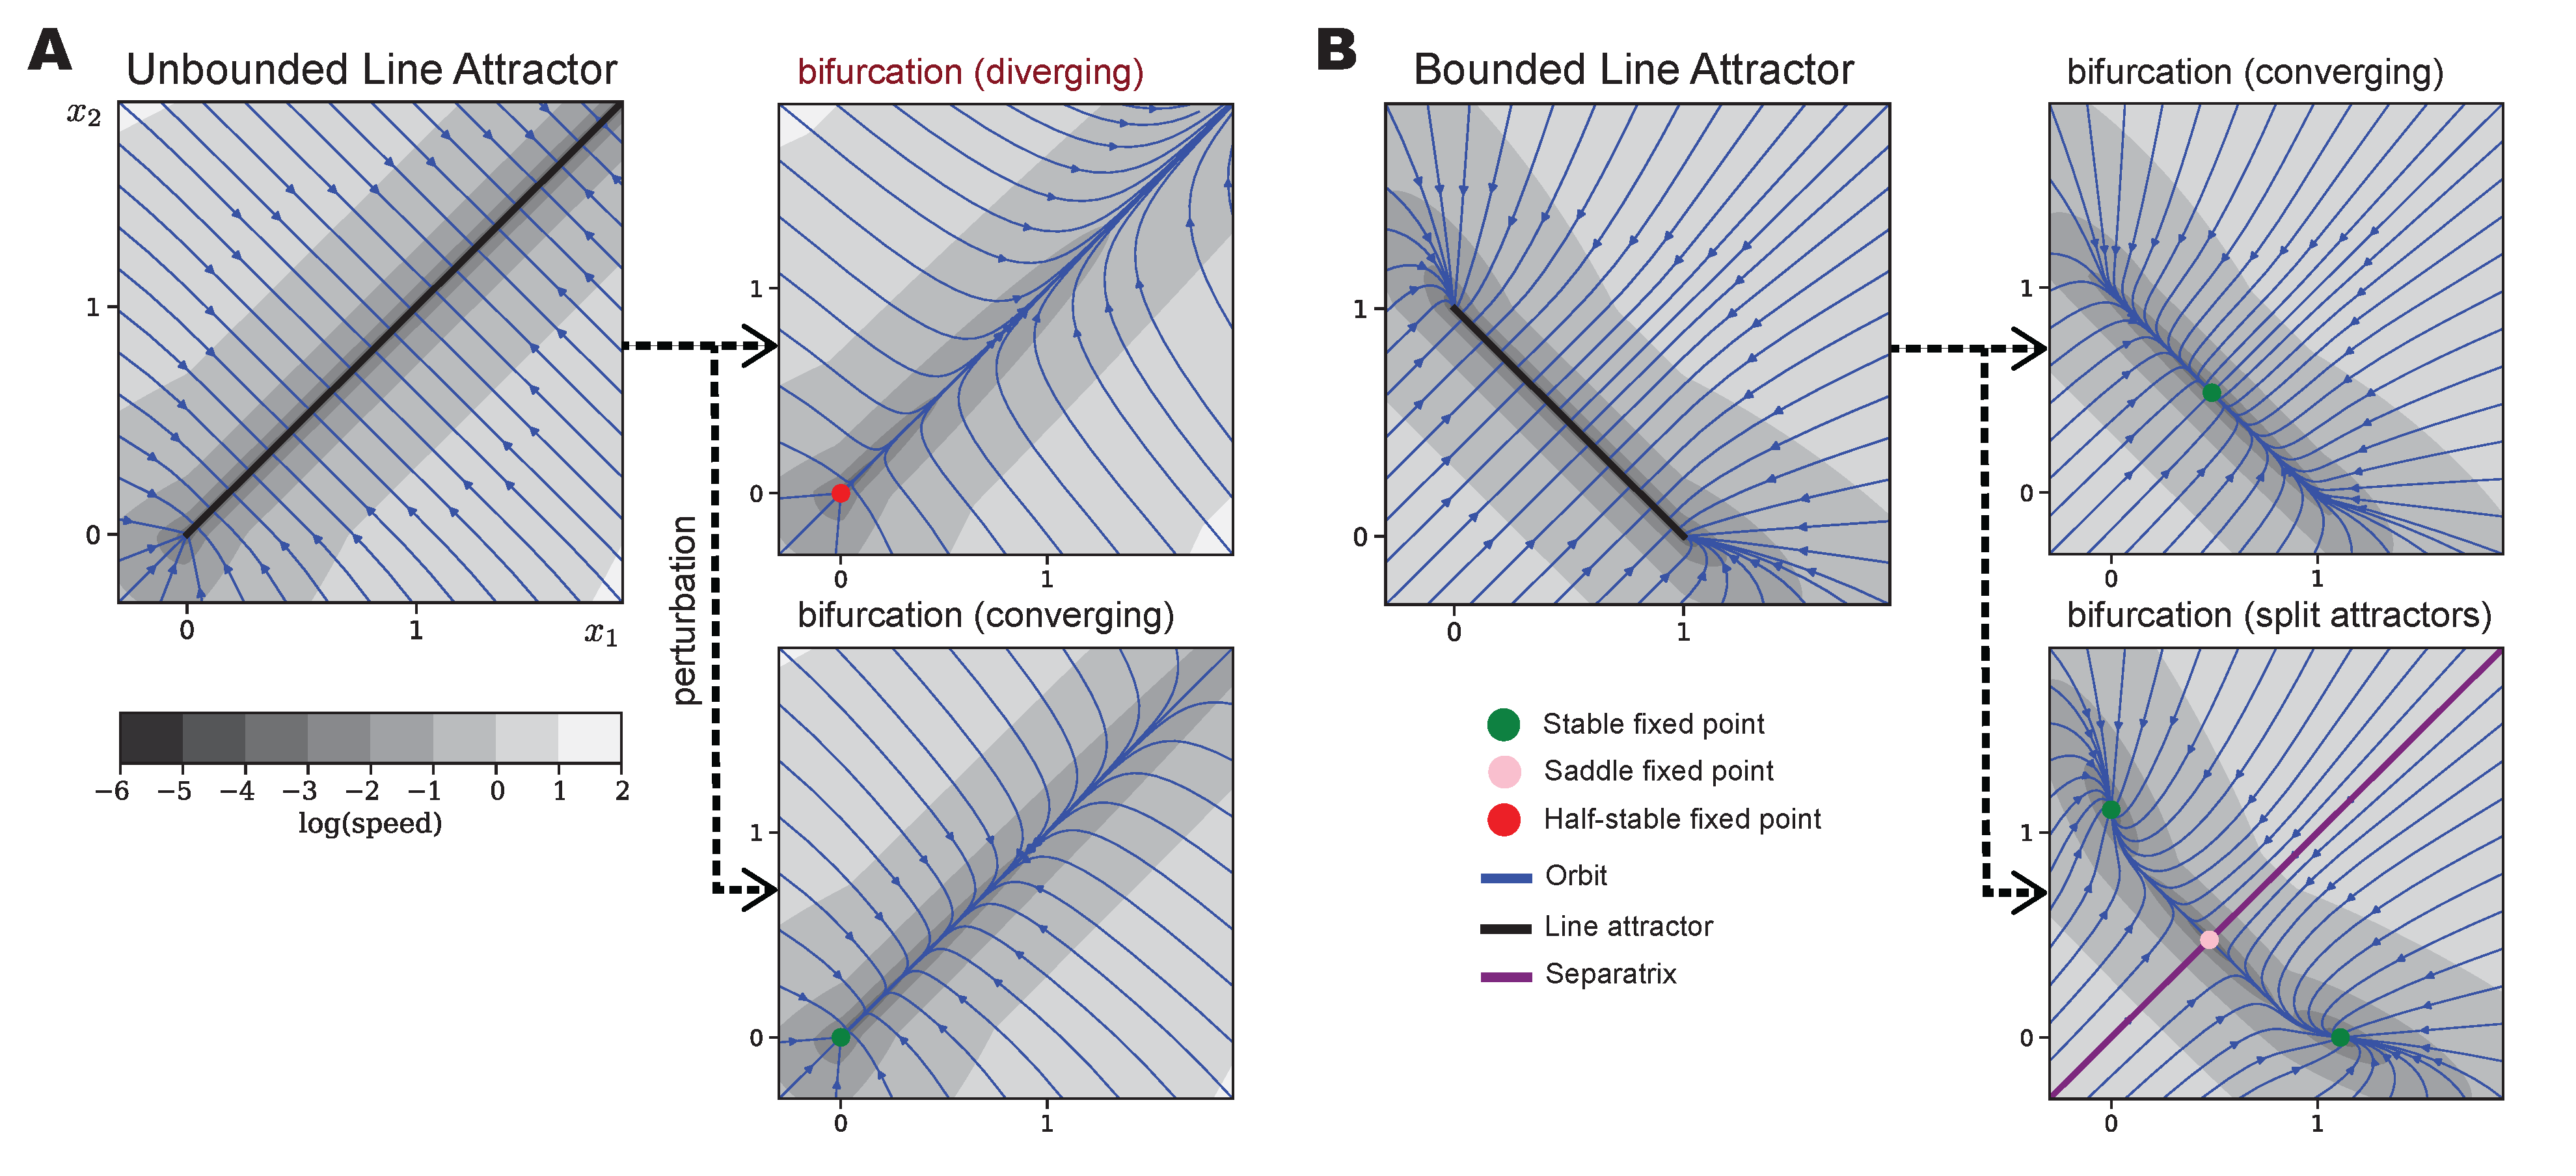
\includegraphics[width=\textwidth]{UBLABLA}
  \caption{Motivating case study of the two systems implementing the same computation but one near exploding gradients.
    Phase portraits for unbounded and bounded linear attractors~\eqref{eq:TLN}.
    Under perturbation of parameters, each of them can bifurcate to one of the two potential systems without the continuous line attractor.
    Note that the parameters for the UBLA are near a diverging system associated with exploding gradient behavior.
}
  \label{fig:ublabla}
\end{figure}


\newpage
\section{Tasks}
\subsection{The auditory clicks task}
\begin{figure}[H]
    \centering
    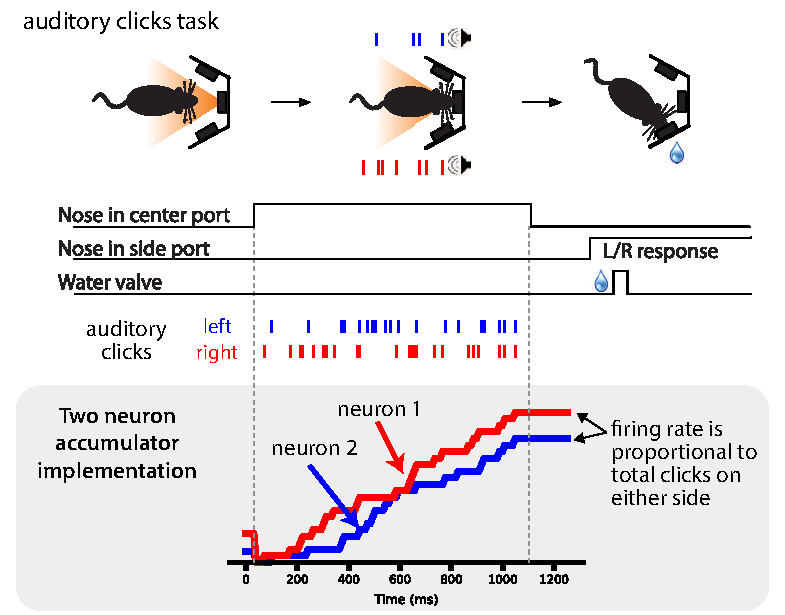
\includegraphics{figures/task_pi_v1.pdf}
    \caption{\textbf{The auditory clicks task and a simple neural network implementation of an accumulator for this task.}
    (Upper part, adapted from [18].) % 
    The sequence of events in each trial is as follows. 
    After light onset rats place their nose into the port and fixate their nose there until the light is turned off. 
    Trains of randomly timed clicks are played concurrently from left and right speakers.
    After nose fixation and sounds ends, the rat makes a choice, poking in the left or the right port to indicate which side played more clicks.
    (In gray box.) There are many ways to implement this auditory task with a Recurrent Neural Network (RNN). In this illustrative example, the firing rates of artificial neurons that can produce appropriate choice behavior for the above auditory task are shown over time. It has two neurons, each counting the number of clicks for one of the sides. The firing rate of one neuron is proportional to the number of clicks on one the sides. The output, i.e., the decision which side to move to, is decided made on which of the neurons has a higher activity.  }%mention input mapping? 
    \label{fig:task_pi_v1}
\end{figure}


\subsection{The angular velocity integration task}
\begin{figure}[H]
    \centering
    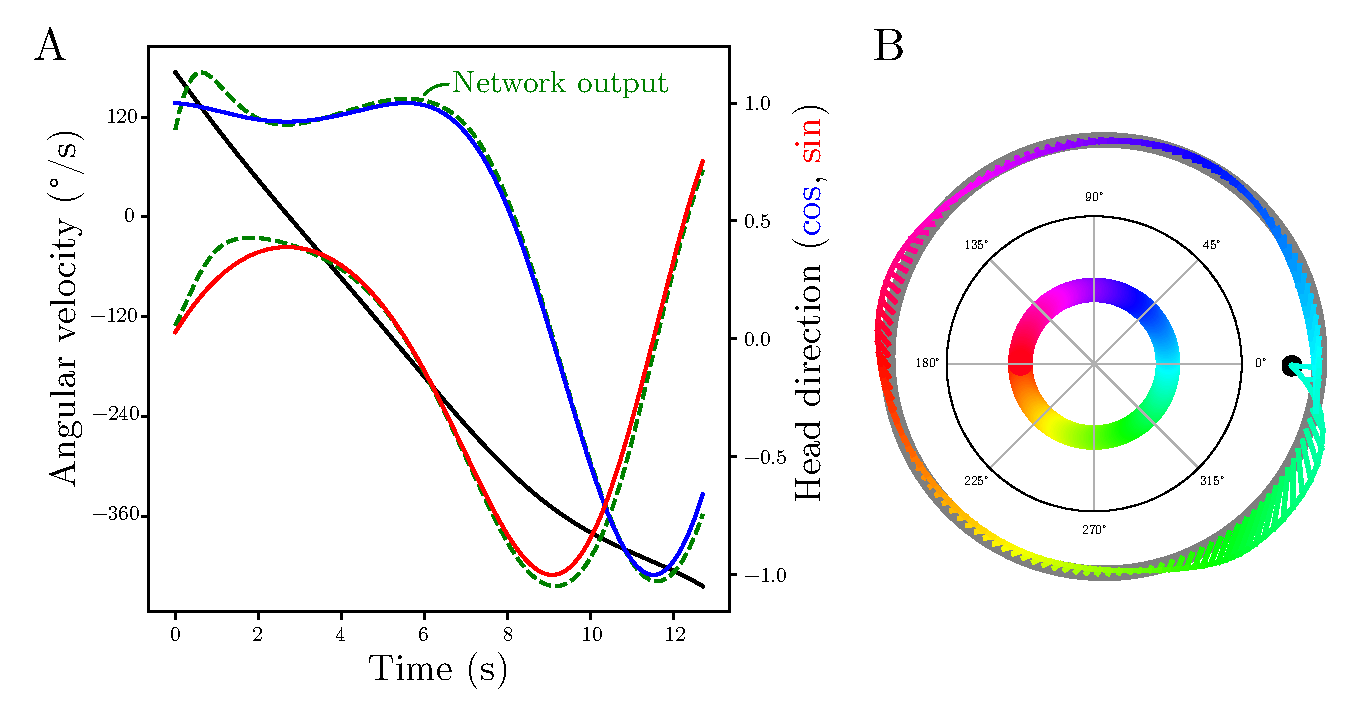
\includegraphics[width=\textwidth]{figures/angular_task.pdf}
    \caption{\textbf{Angular velocity integration task.}
    \textbf{A.} The angular velocity integration task involves integrating angular velocity data over time to obtain angular displacement or orientation information.
    Each sequence consists of input-output pairs, where the input is a sequence of velocities generated by a Gaussian Process, and the output is the target sequence (black line), which corresponds to the integrated angular velocity encoded as the sine and cosine of the angle (blue and red lines respectively), from a random initial position along the circle.
    An example of a trained RNN performing the task is shown (green dashed line).
    \textbf{B.} The output is show in the plane with the difference indicated with lines connecting to the perfect output.
    }
    \label{fig:angular_task}
\end{figure}


\newpage
\section{Slow manifolds}
\subsection{Line}
\begin{figure}[H]
    \centering
    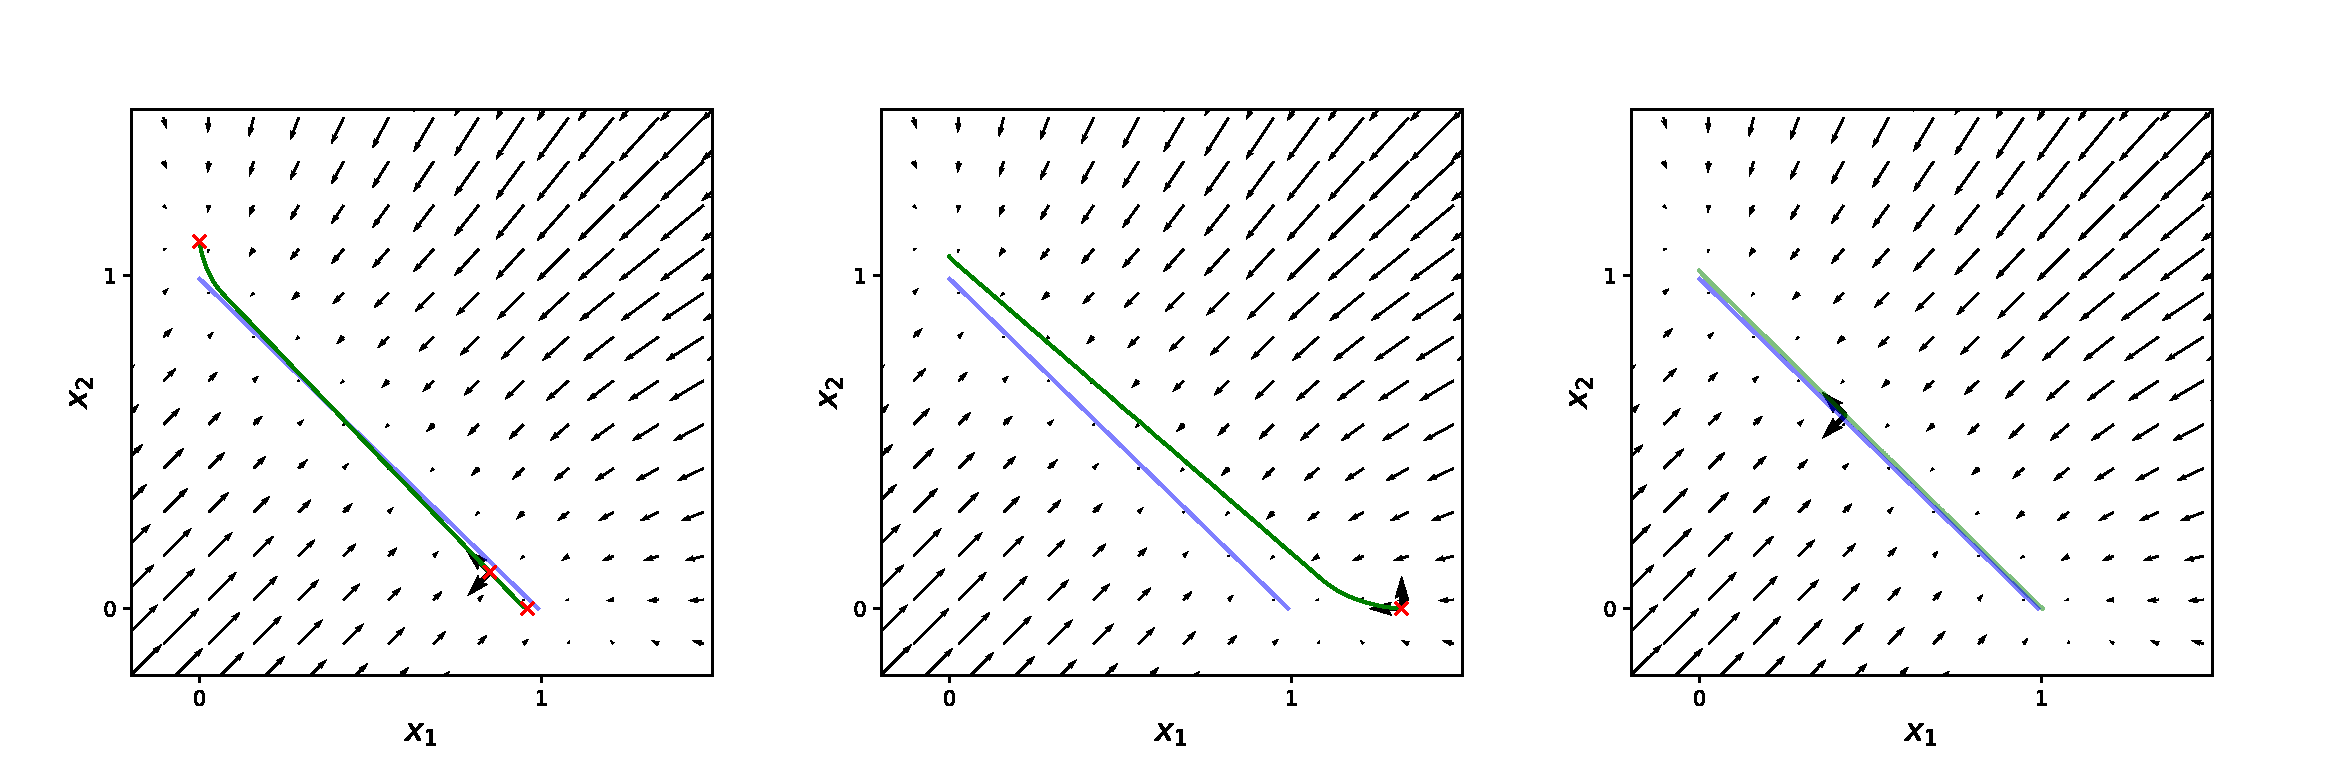
\includegraphics[width=\textwidth]{figures/bla_slowmanifolds.pdf}
    \caption{\textbf{.}}
    \label{fig:}
\end{figure}



\subsection{Ring}
\begin{figure}[htbp]
    \centering
    \begin{subfigure}[b]{0.45\textwidth}
        \centering
        \includegraphics[width=\textwidth]{figures/angular_N100_recttanh_slow_manifold_3d2d}
        \caption{Angular velocity integration task.}
        \label{fig:slowangular}
    \end{subfigure}
    \quad
    \begin{subfigure}[b]{0.45\textwidth}
        \centering
            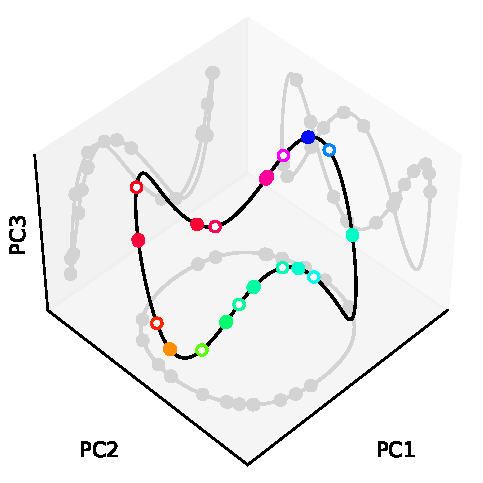
\includegraphics[width=\textwidth]{figures/centerout_N100_tanh_slow_manifold_3d2d.pdf}
        \caption{Memory guided saccade task.}
    \label{fig:slowcenterout}
    \end{subfigure}
    \caption{\textbf{Slow ring manifolds.}}
    \label{fig:slowmanifolds}
\end{figure}



%
%\newpage
%\section{Other examples of neural network implementations of accumulation}
%Here follow some examples of dynamical systems that can correctly perform the auditory task as described in Figure \ref{fig:task_pi_v1}.
%
%
%\subsection{Line attractor}\label{sec:la}
%
%Equation \ref{eq:la} determines a prefect accumulator whose dynamics is shown in Figure \ref{fig:la}, which is an  example of a continuous attractor.
%
%% Def ODE:
%\begin{align}\label{eq:la}
%\begin{split}
%        \dot x_1 &= -x_1 + x_2\\
%        \dot x_2 &= x_1 - x_2
%\end{split}
%\end{align}
%
%
%\begin{figure}[H]
%    \centering
%    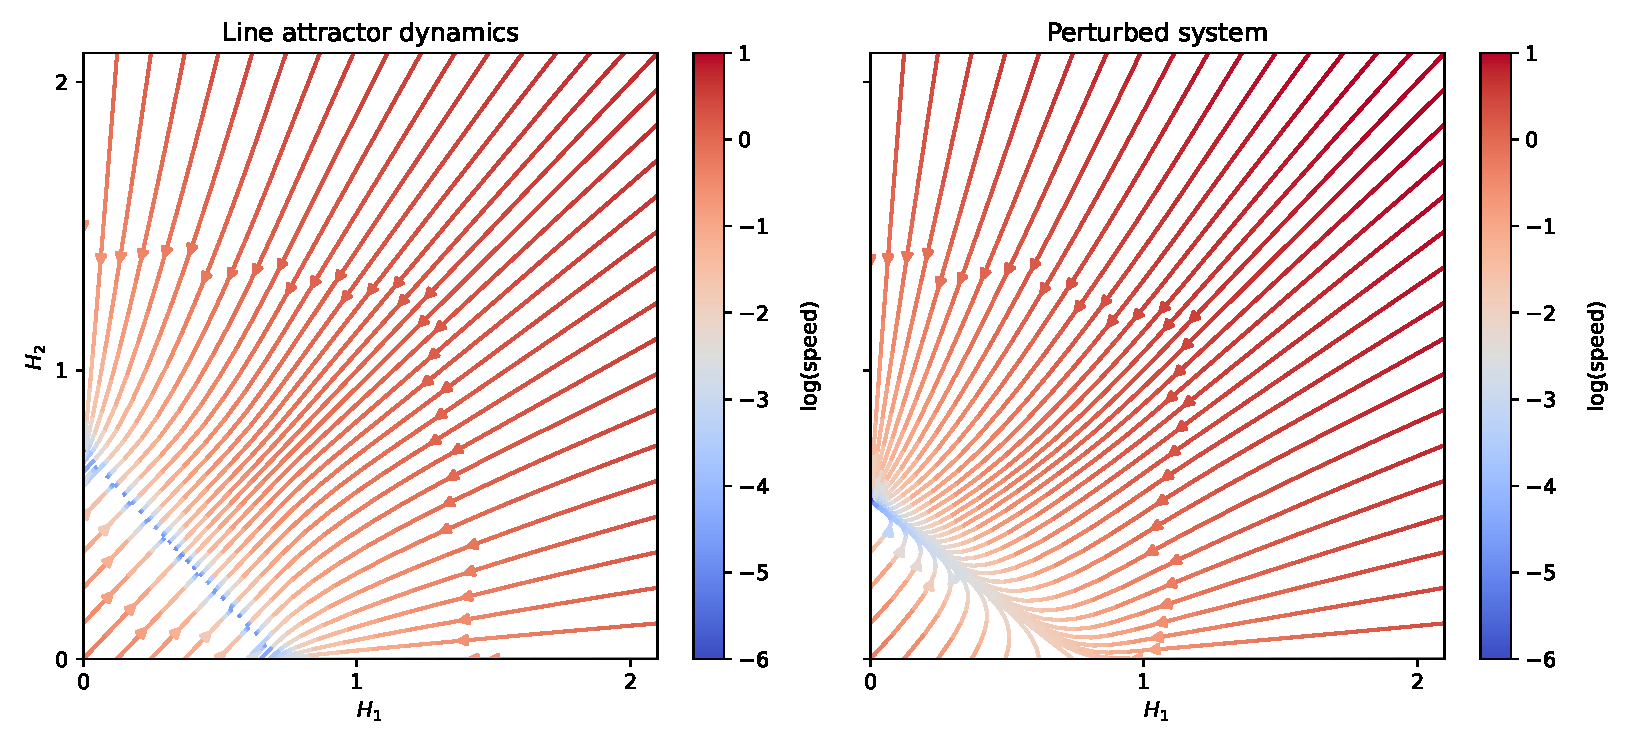
\includegraphics[width=0.99\textwidth]{figures/lineattractor.pdf}
%    \caption{An example of an implementation of a perfect accumulator. This network, composed of two neurons that mutually inhibit each other, achieves the representation of any click difference as a fixed point on the diagonal for each difference. The diagonal is composed of a continuum of fixed points, forming a line attractor. The inputs, i.e., the left and right clicks push the network either to the left or right, respectively, along the diagonal. The correct output, i.e., decision, can be read out from the activity of the neurons being either positive (left choice) or negative (right).
%    \textbf{(Left)} The vector field of the system with the direction shown by the arrows while the magnitude (speed) is shown by the color gradient, yellow for very fast parts and blue for very slow parts, while the white line shows the part of the state space 
%    \textbf{(Right)} The red lines show some example trajectories of the system.}
%    \label{fig:la}
%\end{figure}
%
%% mention: arrow, white 
%
%\newpage
%\subsection{Bounded line attractor}\label{sec:bla}
%Equation \ref{eq:bla} determines a bounded accumulator whose dynamics is shown in Figure \ref{fig:bla}. The $\relu$ activation 
%\begin{align}\label{eq:bla}
%\begin{split}
%        \dot x_1 &= -x_1 + \relu(-x_2 + 1)\\
%        \dot x_2 &= -x_2+ \relu(-x_1 + 1)
%\end{split}
%\end{align}
%\begin{figure}[H]
%    \centering
%    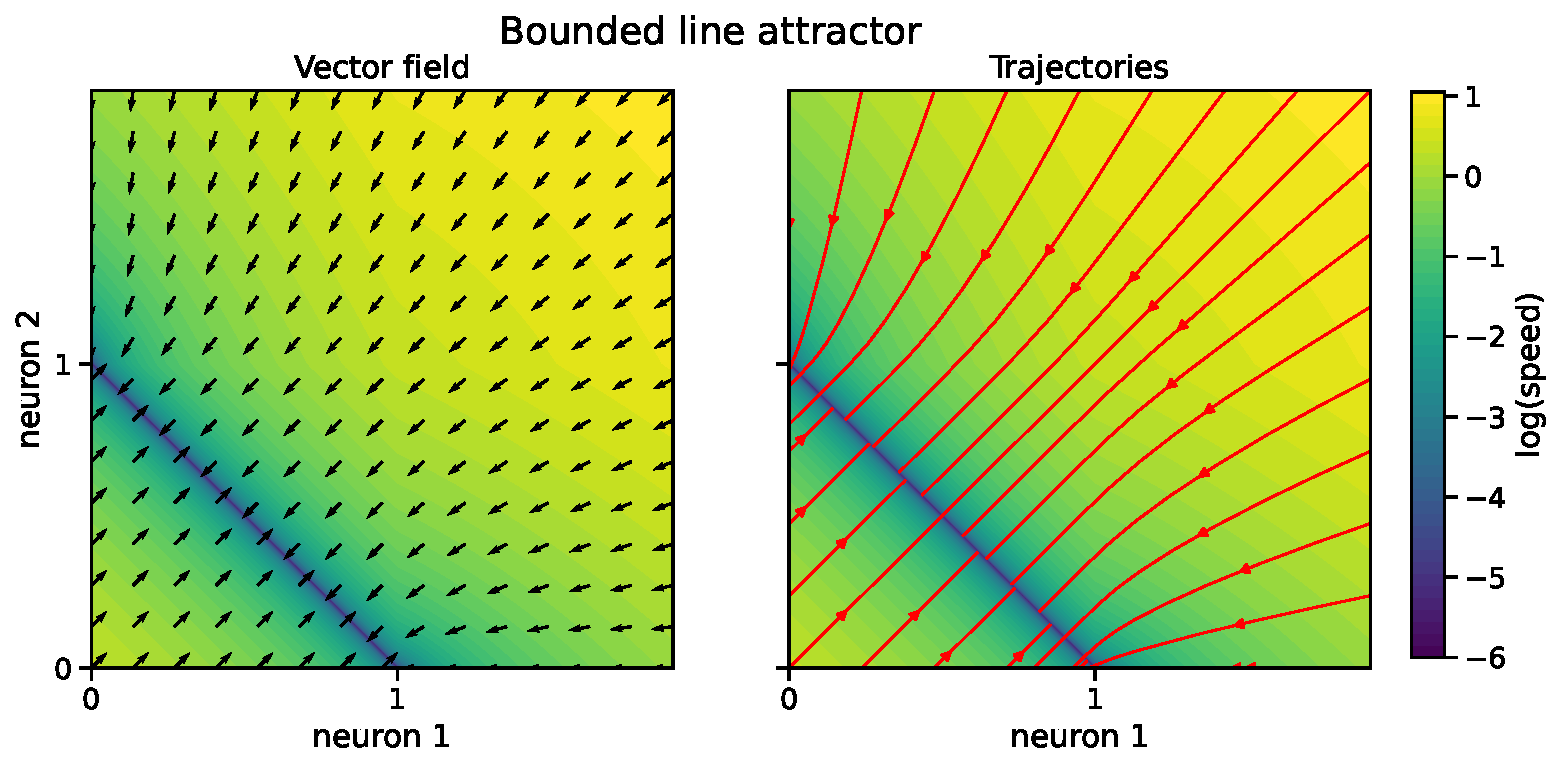
\includegraphics[width=0.99\textwidth]{figures/bounded_lineattractor.pdf}
%    \caption{An example of an implementation of a bounded accumulator. This network represents any click difference by fixed points on the line attractor on the anti-diagonal. 
%    \textbf{(Left)} The vector field of the system with the direction shown by the arrows while the magnitude (speed) is shown by the color gradient, yellow for very fast parts and blue for very slow parts.
%    \textbf{(Right)} The red lines show some example trajectories of the system.}
%    \label{fig:bla}
%\end{figure}
%
%
%\newpage
%\section{Behavior of trained Recurrent Neural Networks (RNNs)}
%
%%Schematic of RNN?
%
%
%
%
%\begin{figure}[H]
%\begin{subfigure}[t]{0.45\linewidth}
%    \centering
%    \includegraphics[width=0.99\textwidth]{figures/hidden_activity_N30_delay.pdf} 
%    \caption{Number of units: $N=30$. This network achieves the integration task by having two fixed points. Which one is reached depends on the click difference during the trials. The fixed point corresponding to the }
%    \label{fig:hidden_activity_N30}
%\end{subfigure}\hfil
%\begin{subfigure}[t]{0.45\linewidth}
%    \centering
%    \includegraphics[width=0.99\textwidth]{figures/hidden_activity_N100_delay.pdf} 
%    \caption[b]{Number of units: $N=100$. This network achieves the integration task by having at least four fixed points. One of the fixed point corresponds to trials where the difference between the number of clicks on the left and right is zero. Two of the fixed points encode the situation where more clicks were presented on the left. Finally, the remaining fixed point encodes trials with more clicks on the right.}
%    \label{fig:hidden_activity_N100}
% \end{subfigure}
% \caption{Two examples of trained RNNs on the auditory task with qualitatively different long-term dynamics.
% The neural activity of a single unit for different trials is shown throughout the trial.
% The clicks start at 100ms while the output cue is presented at 1500ms.
% The trials are colored by the overall click difference during the trial, red where the number of clicks on the right was more than on the left, and blue for the reversed situation. }
%\end{figure}
%
%
%\newpage 
%\section{Perturbation and robustness}
%
%%two points
%%different approximations of cont attractor
%
%%different perturbed systems around CA
%
%
%
%
%\begin{figure}[H]
%    \centering
%    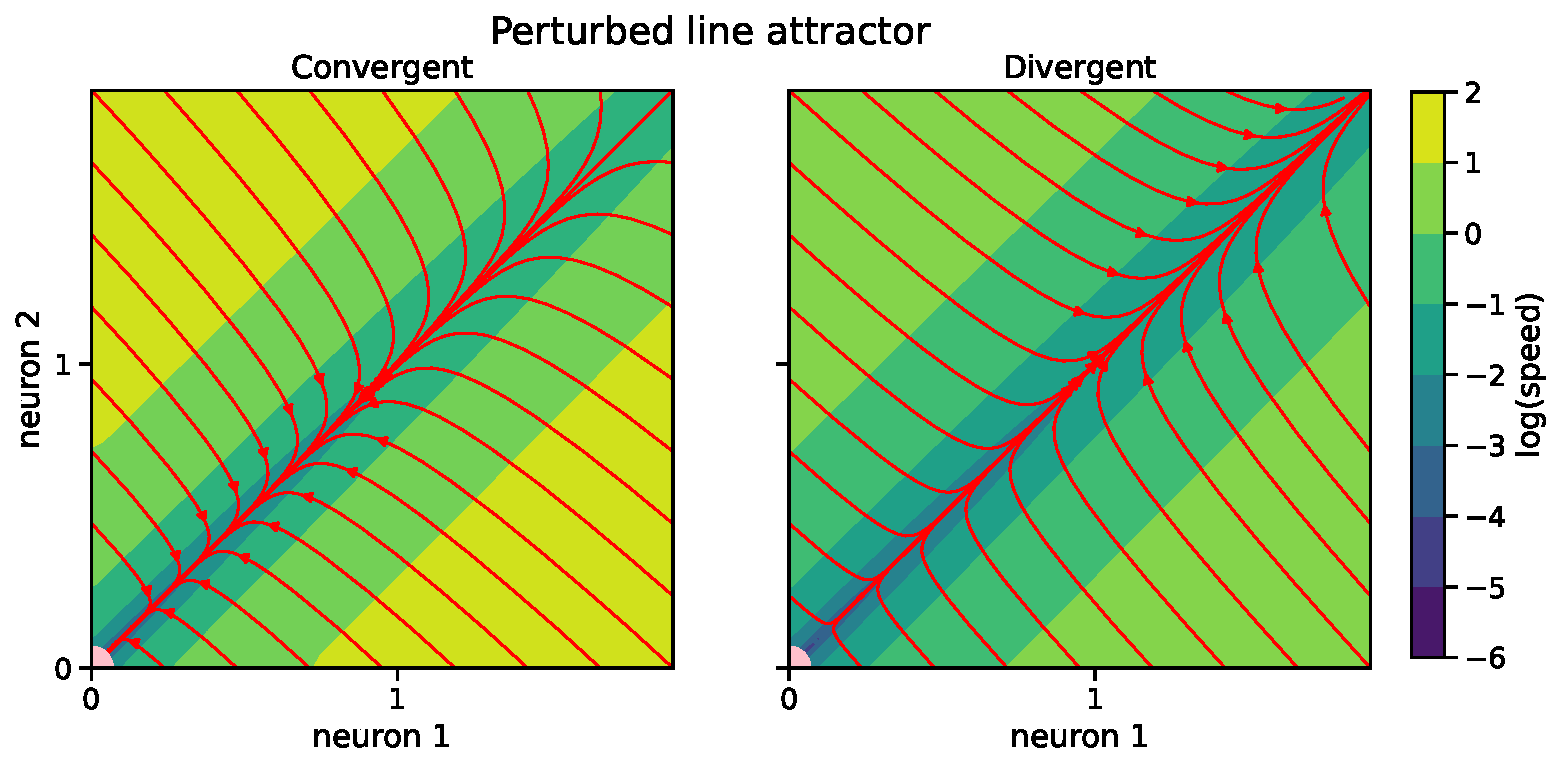
\includegraphics[width=0.99\textwidth]{figures/lineattractor_pert2.pdf}
%    \caption{Two examples of perturbations to the line attractor system in Section \ref{sec:la} with qualitatively different dynamics. These can be seen as two approximations of this continuous attractor. However, the system on the left has very different long-term behavior as it has a stable fixed point at the origin and trajectories converging to it, while the system on the right has an unstable fixed point and divergent trajectories.}
%    \label{fig:perturbed_la}
%\end{figure}
%
%%look at that: some of the perturbations lead to divergent dynamics!
%
%
%% Params: 
% % W_hh =[[ 0.07494547  0.8713927 ]
% % [ 0.85154349 -0.36533186]]
% % b = [-8.28462937e-05 -3.19631364e-03]
%
% %  W_hh =[[ 0.28766126  1.21158179]
% % b = [ 1.08302499 -0.25117677]] [-8.28462937e-05 -3.19631364e-03]
%
%
%\begin{figure}[H]
%    \centering
%    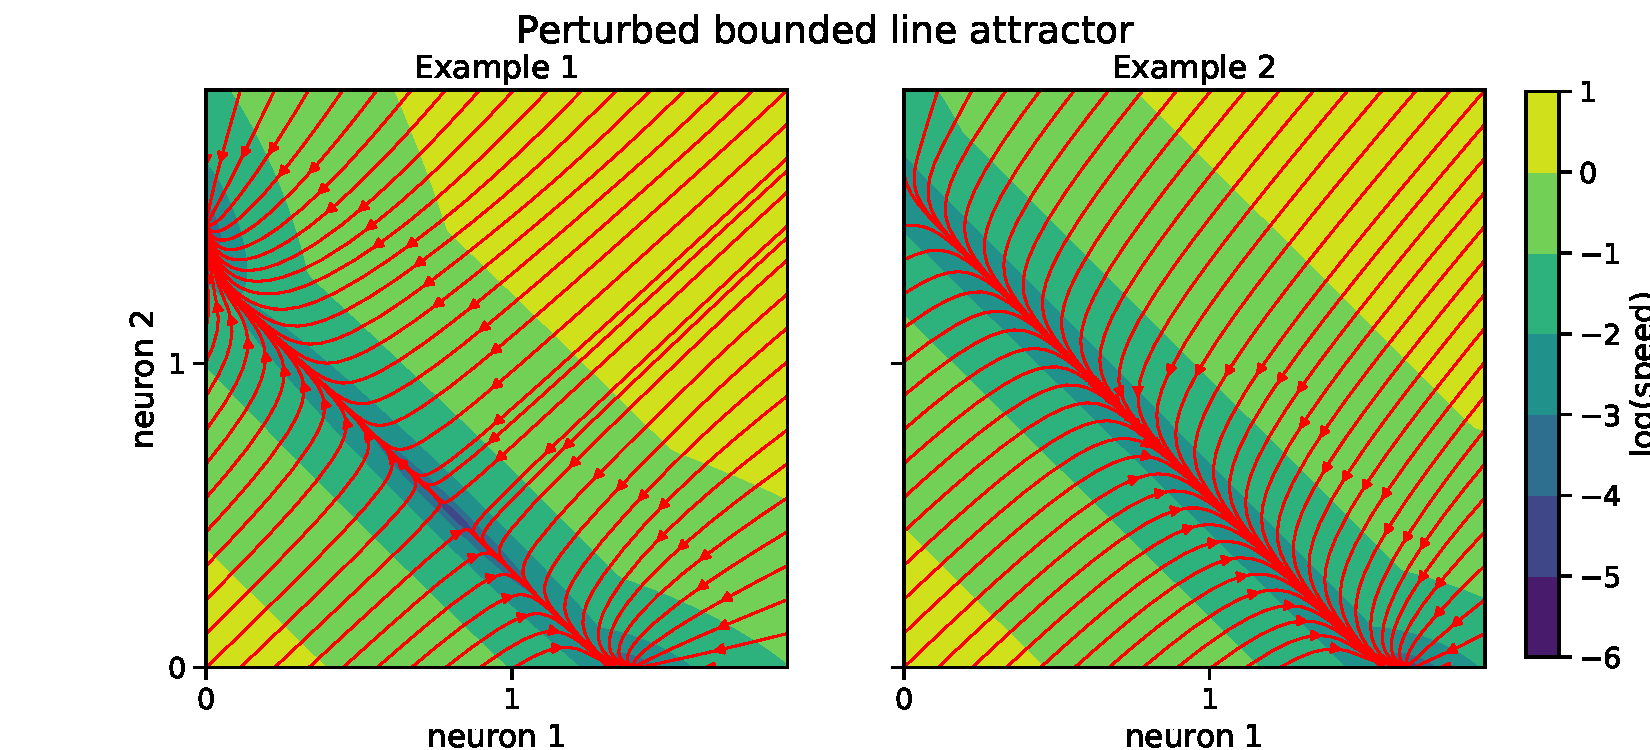
\includegraphics[width=0.99\textwidth]{figures/bounded_lineattractor_pert2.pdf}
%    \caption{Two examples of perturbations to the line attractor system in Section \ref{sec:bla} with qualitatively different dynamics.
%    Also, note that unlike the perturbation on the right in Figure \ref{fig:perturbed_la} none of the perturbations to this system lead to divergent behavior.}
%    \label{fig:perturbed_bla}
%\end{figure}





\newpage
\section{Overview of project}
\begin{figure}[H]
    \centering
    \includegraphics[width=0.99\textwidth]{figures/abstraction_aims_n.pdf}
    \caption{The aims of the project shown with the different levels of abstraction for neural dynamics they correspond to. 
    Every single initialization of a dynamical system, such as the brain or an RNN, and every input sequence leads to a unique trajectory, so identifying each possible sequence should fully describe the input-output mapping.
    However, as the state space and the temporal input space of an RNN is typically big, and we lack a general theory of RNN dynamics, it is very time consuming to simulate all the possible trajectories and for humans it is impossible to all consider them.
    Some trajectories, even though they differ initially, might all converge onto the same point (which is called a \emph{stable fixed point}), where they then remain forever.
    This process abstracts both spatially (different points converge to the fixed point are considered equivalent) and temporally (we can represent the trajectory as a single point). To find these structures automatically is the main goal of \textbf{Aim 1}.
    The general theory through which we can characterize the global dynamics of a dynamical system relies on all kinds of structure for the trajectories, such as fixed points, limit cycles, chaotic orbits and connecting orbits.
    How these are all connected through transient trajectories gets captured in a Morse graph. An adjusted version will be developed for \textbf{Aim 2}.
    As these graphs might be too complex, we need an interpretable version of it, that might for example be seen as an approximation to a continuous attractor. This simplification step is the main focus of \textbf{Aim 3}.
    }
    \label{fig:abstraction_aims}
\end{figure}



% \newpage
% \section{Morse decomposition}
% \begin{figure}[H]
%     \centering
% \begin{tikzpicture}[scale=2]
% \pgfmathsetmacro{\shift}{0.25ex}
% \node (1) at (-0.5,3) {$M(1)$};
% \node (2) at (0.5,3) {$M(2)$};
% \node  (3) at (0,2) {$M(3)$};
% % \node [draw , circle] (4) at (0,0) {$4$};
% % \node [draw , circle] (5) at (0.5,1) {$5$};
% % \node [draw , circle] (6) at (-0.5,1) {$6$};
% % \draw [->] (1) -- (2);
% % \draw [->,shorten <=-1pt, transform canvas={xshift=-\shift,yshift=-\shift}] (1) -- (3);
% \draw [->,shorten <=-1pt, transform canvas={xshift=\shift,yshift=\shift}] (3) -- (1);
% \draw [->] (3) -- (2);
% \end{tikzpicture}
%     \caption{Morse graph of the networks.  The three Morse sets are the fixed points of the system.}
%     \label{fig:morsegraph1}
% \end{figure}

% \begin{figure}[H]
%     \centering
% \begin{tikzpicture}[scale=2]
% \pgfmathsetmacro{\shift}{0.25ex}
% \node (1) at (0,3) {$M(1)$};
% \node (2) at (0,2) {$M(2)$};
% \draw [->,shorten <=-1pt, transform canvas={xshift=\shift,yshift=\shift}] (2) -- (1);
% \end{tikzpicture}
%     \caption{Morse graph of another network solution (not yet shown).}
%     \label{fig:morsegraph2}
% \end{figure}


% \begin{figure}[H]
%     \centering
% \begin{tikzpicture}[scale=2]
% \pgfmathsetmacro{\shift}{0.25ex}
% \node (1) at (-1,3) {$M(1)$};
% \node (2) at ( 1,3) {$M(2)$};
% \node  (3) at (0,3) {$M(3)$};
% \node  (4) at (0,2) {$M(4)$};
% \draw [->,shorten <=-1pt, transform canvas={xshift=\shift,yshift=\shift}] (4) -- (1);
% \draw [->] (4) -- (2);
% \draw [->] (4) -- (3);
% \end{tikzpicture}
%     \caption{Morse graph of another network solution, see Figure \ref{fig:hidden_activity_N100}}
%     \label{fig:morsegraph3}
% \end{figure}

% \begin{figure}[H]
%     \centering
% \begin{tikzpicture}[scale=2]
% \pgfmathsetmacro{\shift}{0.25ex}
% \node (1) at (-0.5,3) {$M(1)$};
% \node (2) at (0.5,3) {$M(2)$};
% \node  (3) at (0,2) {$M(3)$};
% \node (4) at (-0.5,4) {$Left$};
% \node  (5) at (0.5,4) {$Right$};
% \draw [->,shorten <=-1pt, transform canvas={xshift=\shift,yshift=\shift}] (3) -- (1);
% \draw [->] (3) -- (2);
% \draw [->] (1) -- (4);
% \draw [->] (2) -- (5);
% \end{tikzpicture}
%     \caption{The output mapping of the Morse sets.}
%     \label{fig:morsegraph_outputs1}
% \end{figure}





\end{document}